\documentclass{standalone}
\usepackage{tikz}
\usetikzlibrary{patterns, positioning}


\begin{document}
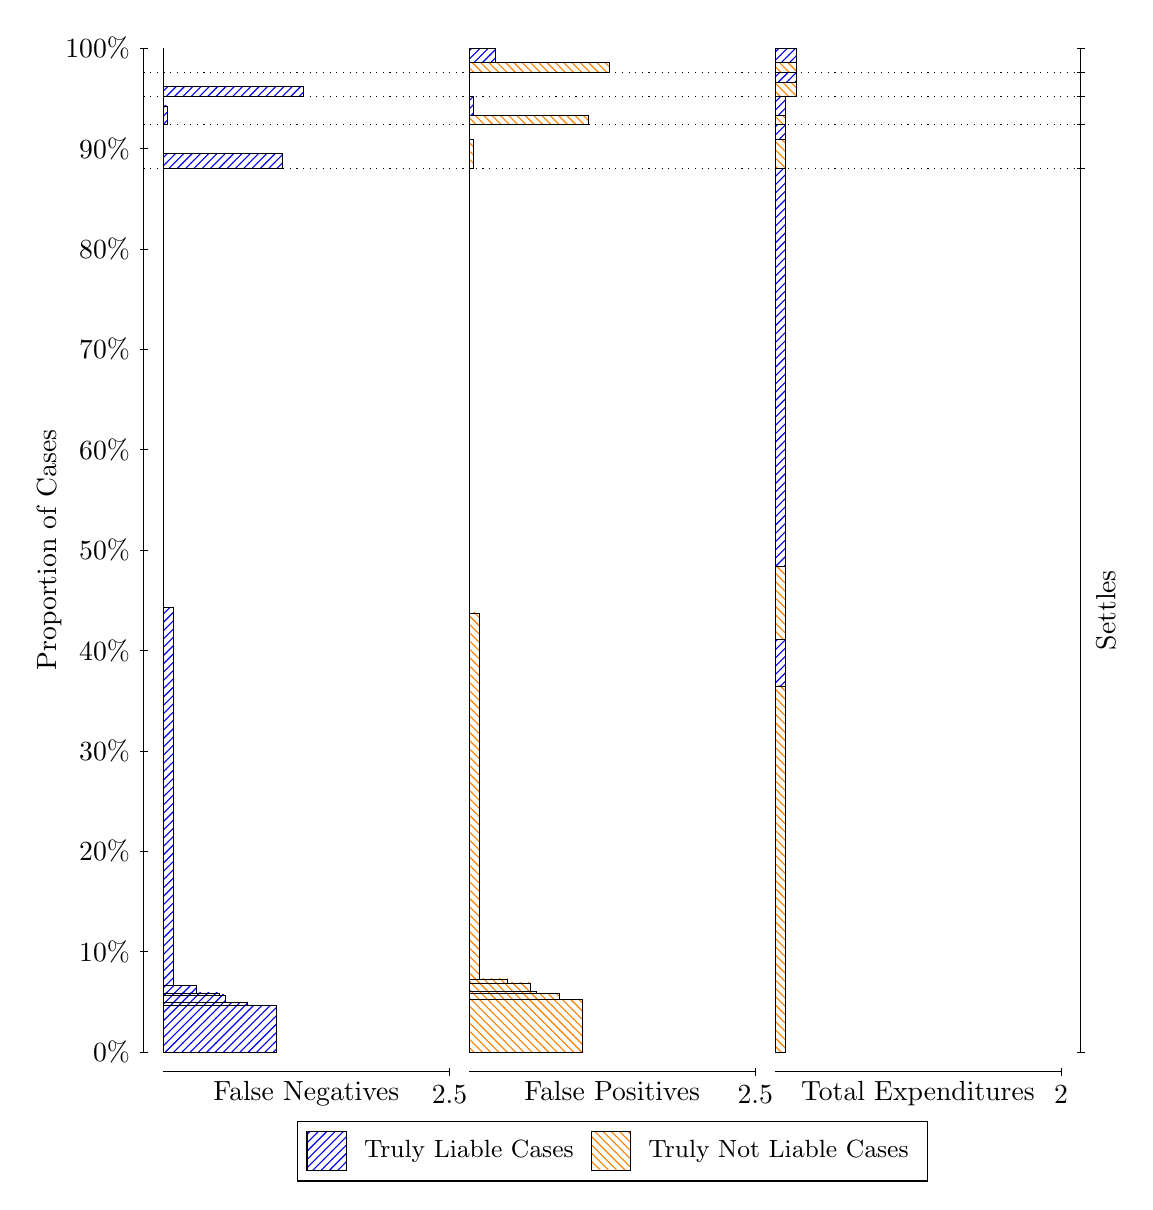
\begin{tikzpicture}
\draw[black, very thin] (1.5,1.75) -- (1.5,14.5);
\node[rotate=90, text=black, anchor=center] at (0.3, 8.125) {Proportion of Cases};
\draw[black, very thin] (1.45,1.75) -- (1.55,1.75);
\node[text=black, anchor=east] at (1.45, 1.75) {0\%};
\draw[black, very thin] (1.45,3.025) -- (1.55,3.025);
\node[text=black, anchor=east] at (1.45, 3.025) {10\%};
\draw[black, very thin] (1.45,4.3) -- (1.55,4.3);
\node[text=black, anchor=east] at (1.45, 4.3) {20\%};
\draw[black, very thin] (1.45,5.575) -- (1.55,5.575);
\node[text=black, anchor=east] at (1.45, 5.575) {30\%};
\draw[black, very thin] (1.45,6.85) -- (1.55,6.85);
\node[text=black, anchor=east] at (1.45, 6.85) {40\%};
\draw[black, very thin] (1.45,8.125) -- (1.55,8.125);
\node[text=black, anchor=east] at (1.45, 8.125) {50\%};
\draw[black, very thin] (1.45,9.4) -- (1.55,9.4);
\node[text=black, anchor=east] at (1.45, 9.4) {60\%};
\draw[black, very thin] (1.45,10.675) -- (1.55,10.675);
\node[text=black, anchor=east] at (1.45, 10.675) {70\%};
\draw[black, very thin] (1.45,11.95) -- (1.55,11.95);
\node[text=black, anchor=east] at (1.45, 11.95) {80\%};
\draw[black, very thin] (1.45,13.225) -- (1.55,13.225);
\node[text=black, anchor=east] at (1.45, 13.225) {90\%};
\draw[black, very thin] (1.45,14.5) -- (1.55,14.5);
\node[text=black, anchor=east] at (1.45, 14.5) {100\%};

\draw[black, very thin] (13.4,1.75) -- (13.4,14.5);
\draw[black, very thin] (13.35,1.75) -- (13.45,1.75);
\node[anchor=west] at (13.35, 1.75) {};
\draw[black, very thin] (13.35,12.973) -- (13.45,12.973);
\node[anchor=west] at (13.35, 12.973) {};
\draw[black, very thin] (13.35,13.529) -- (13.45,13.529);
\node[anchor=west] at (13.35, 13.529) {};
\draw[black, very thin] (13.35,13.885) -- (13.45,13.885);
\node[anchor=west] at (13.35, 13.885) {};
\draw[black, very thin] (13.35,14.193) -- (13.45,14.193);
\node[anchor=west] at (13.35, 14.193) {};
\draw[black, very thin] (13.35,14.5) -- (13.45,14.5);
\node[anchor=west] at (13.35, 14.5) {};

\draw[black, very thin, pattern color=blue, pattern=north east lines] (1.75,1.75) rectangle (3.1852,2.341);
\draw[black, very thin, pattern color=blue, pattern=north east lines] (1.75,2.341) rectangle (2.8218,2.3755);
\draw[black, very thin, pattern color=blue, pattern=north east lines] (1.75,2.3755) rectangle (2.5312,2.4745);
\draw[black, very thin, pattern color=blue, pattern=north east lines] (1.75,2.4745) rectangle (2.4585,2.5001);
\draw[black, very thin, pattern color=blue, pattern=north east lines] (1.75,2.5001) rectangle (2.1678,2.5937);
\draw[black, very thin, pattern color=blue, pattern=north east lines] (1.75,2.5937) rectangle (1.8772,7.396);
\draw[black, very thin, pattern color=orange, pattern=north west lines] (1.75,7.396) rectangle (1.75,12.973);
\draw[black, very thin, pattern color=blue, pattern=north east lines] (1.75,12.973) rectangle (3.2578,13.158);
\draw[black, very thin, pattern color=orange, pattern=north west lines] (1.75,13.158) rectangle (1.75,13.529);
\draw[black, very thin, pattern color=blue, pattern=north east lines] (1.75,13.529) rectangle (1.8045,13.766);
\draw[black, very thin, pattern color=orange, pattern=north west lines] (1.75,13.766) rectangle (1.75,13.885);
\draw[black, very thin, pattern color=blue, pattern=north east lines] (1.75,13.885) rectangle (3.5303,14.01);
\draw[black, very thin, pattern color=orange, pattern=north west lines] (1.75,14.01) rectangle (1.75,14.193);
\draw[black, very thin, pattern color=orange, pattern=north west lines] (1.75,14.193) rectangle (1.75,14.318);
\draw[black, very thin, pattern color=blue, pattern=north east lines] (1.75,14.318) rectangle (1.75,14.5);
\draw[black, very thin, pattern color=orange, pattern=north west lines] (5.6333,1.75) rectangle (7.0685,2.421);
\draw[black, very thin, pattern color=orange, pattern=north west lines] (5.6333,2.421) rectangle (6.7778,2.4909);
\draw[black, very thin, pattern color=orange, pattern=north west lines] (5.6333,2.4909) rectangle (6.4872,2.5165);
\draw[black, very thin, pattern color=orange, pattern=north west lines] (5.6333,2.5165) rectangle (6.4145,2.6271);
\draw[black, very thin, pattern color=orange, pattern=north west lines] (5.6333,2.6271) rectangle (6.1238,2.6775);
\draw[black, very thin, pattern color=orange, pattern=north west lines] (5.6333,2.6775) rectangle (5.7605,7.3268);
\draw[black, very thin, pattern color=blue, pattern=north east lines] (5.6333,7.3268) rectangle (5.6333,12.973);
\draw[black, very thin, pattern color=orange, pattern=north west lines] (5.6333,12.973) rectangle (5.6878,13.344);
\draw[black, very thin, pattern color=blue, pattern=north east lines] (5.6333,13.344) rectangle (5.6333,13.529);
\draw[black, very thin, pattern color=orange, pattern=north west lines] (5.6333,13.529) rectangle (7.1412,13.648);
\draw[black, very thin, pattern color=blue, pattern=north east lines] (5.6333,13.648) rectangle (5.6878,13.885);
\draw[black, very thin, pattern color=orange, pattern=north west lines] (5.6333,13.885) rectangle (5.6333,14.068);
\draw[black, very thin, pattern color=blue, pattern=north east lines] (5.6333,14.068) rectangle (5.6333,14.193);
\draw[black, very thin, pattern color=orange, pattern=north west lines] (5.6333,14.193) rectangle (7.4137,14.318);
\draw[black, very thin, pattern color=blue, pattern=north east lines] (5.6333,14.318) rectangle (5.9603,14.5);
\draw[black, very thin, pattern color=orange, pattern=north west lines] (9.5167,1.75) rectangle (9.6529,6.3992);
\draw[black, very thin, pattern color=blue, pattern=north east lines] (9.5167,6.3992) rectangle (9.6529,6.9903);
\draw[black, very thin, pattern color=orange, pattern=north west lines] (9.5167,6.9903) rectangle (9.6529,7.9178);
\draw[black, very thin, pattern color=blue, pattern=north east lines] (9.5167,7.9178) rectangle (9.6529,12.973);
\draw[black, very thin, pattern color=orange, pattern=north west lines] (9.5167,12.973) rectangle (9.6529,13.344);
\draw[black, very thin, pattern color=blue, pattern=north east lines] (9.5167,13.344) rectangle (9.6529,13.529);
\draw[black, very thin, pattern color=orange, pattern=north west lines] (9.5167,13.529) rectangle (9.6529,13.648);
\draw[black, very thin, pattern color=blue, pattern=north east lines] (9.5167,13.648) rectangle (9.6529,13.885);
\draw[black, very thin, pattern color=orange, pattern=north west lines] (9.5167,13.885) rectangle (9.7892,14.068);
\draw[black, very thin, pattern color=blue, pattern=north east lines] (9.5167,14.068) rectangle (9.7892,14.193);
\draw[black, very thin, pattern color=orange, pattern=north west lines] (9.5167,14.193) rectangle (9.7892,14.318);
\draw[black, very thin, pattern color=blue, pattern=north east lines] (9.5167,14.318) rectangle (9.7892,14.5);
\draw[black, dotted] (1.5,12.973) -- (13.4,12.973);
\draw[black, dotted] (1.5,13.529) -- (13.4,13.529);
\draw[black, dotted] (1.5,13.885) -- (13.4,13.885);
\draw[black, dotted] (1.5,14.193) -- (13.4,14.193);
\draw[black, very thin] (1.75,1.5) -- (5.3833,1.5);
\node[text=black, anchor=north] at (3.5667, 1.5) {False Negatives};
\draw[black, very thin] (5.3833,1.45) -- (5.3833,1.55);
\node[text=black, anchor=north] at (5.3833, 1.45) {2.5};

\draw[black, very thin] (5.6333,1.5) -- (9.2667,1.5);
\node[text=black, anchor=north] at (7.45, 1.5) {False Positives};
\draw[black, very thin] (9.2667,1.45) -- (9.2667,1.55);
\node[text=black, anchor=north] at (9.2667, 1.45) {2.5};

\draw[black, very thin] (9.5167,1.5) -- (13.15,1.5);
\node[text=black, anchor=north] at (11.333, 1.5) {Total Expenditures};
\draw[black, very thin] (13.15,1.45) -- (13.15,1.55);
\node[text=black, anchor=north] at (13.15, 1.45) {2};

\node[text=black, centered, rotate=90] at (13.72, 7.3614) {Settles};





\draw (7.449999999999999,1.5) node[draw=none] (baseCoordinate) {};
\begin{scope}[align=center]
        \matrix[scale=0.5, draw=black, below=0.5cm of baseCoordinate, nodes={draw}, column sep=0.1cm]{
            \node[rectangle, draw, minimum width=0.5cm, minimum height=0.5cm, pattern color=blue, pattern=north east lines] {}; &
            \node[draw=none, font=\small, text=black] (B) {Truly Liable Cases}; &
            \node[rectangle, draw, minimum width=0.5cm, minimum height=0.5cm, pattern color=orange, pattern=north west lines] {}; &
            \node[draw=none, font=\small, text=black] (B) {Truly Not Liable Cases}; \\
            };
\end{scope}

\end{tikzpicture}
\end{document}